


\chapter[运动预测算法设计]{运动预测算法设计}[Harbin Institute of Technology Postgraduate Dissertation Writing Specifications]


\section{引言}[Content specification]

运动预测本质上是对运动物体的建模,比如,通过观测得到当前物体的位置,
并结合历史观测数据(位置、时间戳等)能够计算出物体的运动信息(如速度、加速度等),
从而能够预测未来在$t$时刻物体的位置,以在一维$x$方向匀速运动的物体为例,其运动学公式见式(3-1),其中$x(t)$表示物理位置随时间的变化,$x_0$表示初位置,$v_x$表示物体在$x$方向上的速度,$t$表示时间。
\begin{gather}
    x(t) = x_0 + v_x*t \label{linear_model}
\end{gather}

对运动物体的建模即为假定一个运动模型,通过历史数据拟合参数。
比如,匀速运动模型为通过一堆带着时间信息的坐标点去拟合速度。




\section{运动模型的坐标系选择}[Content specification]

通过高效透视n点算法(Efficient Perspective-n-Point algorithm, EPnP)算法或者是其他算法解算的目标位置(实际上得到的是位置和姿态,
但是运动预测不需要目标的姿态,因此下文只考虑目标的位置)的坐标系是相机坐标系,但是,
云台运动时相机坐标系的位姿也会有变化,观测的相对于大地静止的目标也会发生变化,这样不利于建立运动模型。所以,
需要将目标的位置坐标转换到惯性坐标系下,这样目标点的位置不随着云台运动而运动,从而可以建立准确的运动学模型。\par
由于设备采用的是单目相机,得到某点的信息只有其在$x$和$y$方向的像素坐标信息,
其实得到是目标相对于相机坐标系的$yaw$和$pitch$轴角度信息,
即,相机成像的物理模型使得在观测物体的位置时选择的坐标系为球坐标系。
至于深度信息,即球半径,单目相机在没有先验知识的情况下是无法结算出的。
然而装甲板的实际尺寸大小是已知的(先验),由透镜成像的物理模型(图\ref{透镜成像模型})可得公式(3-2),其中$d$为物体距离相机光心深度值,$f$为相机焦距,$h$为物体实际高度,$y$为物体成像高度。\par
\begin{gather}
    d = \frac{fh}{y} 
\end{gather}

\begin{figure}[H]
    \centering
    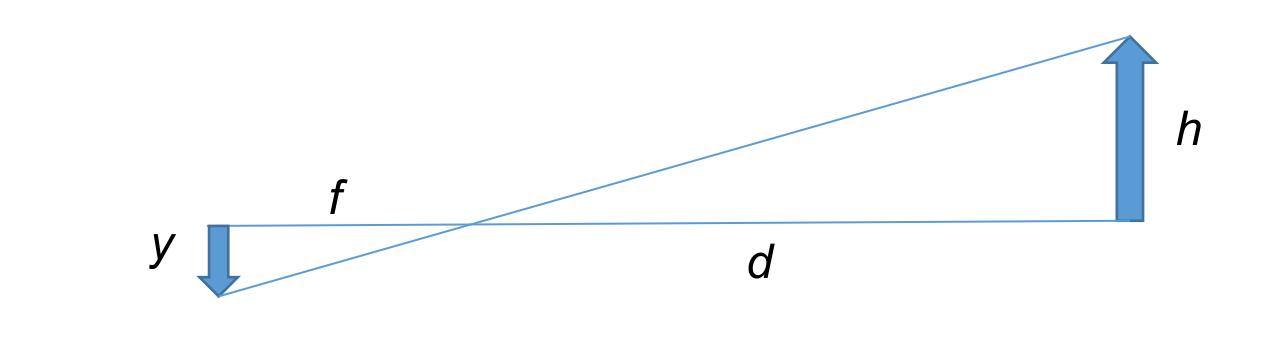
\includegraphics[width=.8\textwidth]{camera_model.png} 
    \caption{透镜成像模型}
    \label{透镜成像模型} 
\end{figure}    
这样,通过计算灯条的像素高度、事先标定好的相机内参中的$f_y$和先验装甲版实际高度就可以计算出目标相对于相机的实际距离。
注意,上面的$y$的单位不是像素,而是$mm$、$m$这样的单位,
而实际从图像上读的是像素值,因此实际的计算见公式(3-3),其中$d_y$为$y$轴像元尺寸,$f_y$为$y$轴的归一化焦距。
\begin{gather}
    d=\frac{fh}{y_{像素}}=\frac{fh}{y*dy}=\frac{f_yh}{y}
\end{gather}
这样,就得到了物体在相机坐标系下的位置描述$(yaw,pitch, distance)$。
当然,可以把它再转换到笛卡尔坐标系$(x,y,z)$。不过需要注意的是,
转换之后的$x,y,z$之间存在耦合关系(例如:$x$、$y$都与$distancce$有关,当$distance$发生改变时,$x$、$y$同时都会改变);
但是$yaw,pitch,distance$之间则相互独立。\par

从计算深度距离$distance$的公式可以看出最大的不确定的因素就是顶点像素的位置,
提取像素点不可能完全的准确。采用图像二值化的方式,提取的轮廓边缘的像素值一定是在阈值附近的,
有时高于阈值,有时低于阈值,影响就是结算出来的距离一直在波动;且随着距离的增加,构成灯条的像素点数减少,像素点的波动对于测距影响增大,影响就是距离越远,测距误差越大。
因为上述所说的噪声不可避免,所以采用卡尔曼滤波器得到深度信息的最优估计值。\par

\section{运动模型选择}[Content specification]
要使用卡尔曼滤波器,我们首先需要确定运动模型。对于运动模型,首先需要明确的是运动模型实际上是无法用数学公式描述的,
即使能够用数学公式描述对于而言也是不可知的。 所以只能假设它是匀速运动模型或者是匀加速运动模型或是其他运动模型。
对于RoboMaster比赛来说,匀速运动模型能够应对大多数场合。然而,机器人加减速频繁,那么选择匀加速模型是不是更准确呢? 
经过测试发现,引入加速度后,从原先只需要拟合一个参数变成了拟合两个参数,容易造成拟合结果的不准确。且容易产生过拟合现象。
如下图所示,高阶模型固然对已有的点拟合的准确,但从图\ref{过拟合现象}中明显可以看出如果新加一个点,必然与拟合的曲线相差甚大。
\begin{figure}[H]
    \centering
    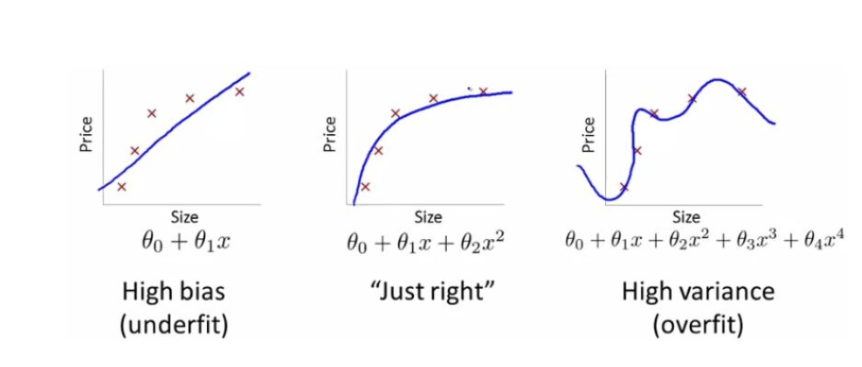
\includegraphics[width=.8\textwidth]{overfit_demo.png} 
    \caption{过拟合现象} 
    \label{过拟合现象} 
\end{figure} 

综上所述,建立的运动模型为$yaw$方向匀速运动,深度方向匀速运动。

\section{基于卡尔曼滤波器建立目标运动模型}[Content specification]

使用卡尔曼滤波器建立物体运动模型过程如下。
\par
将EPnP算法解算出目标在相机坐标系 ($c$系)的坐标$p_c$投影到球坐标系上,见公式(3-4):
\begin{equation} \boldsymbol p_c=\left[\begin{array}{c} yaw_c\\ pitch_c \\ distance_c \end{array}\right] \end{equation}
\par 
通过机械测量得到相机与云台旋转中心的相对位置,则目标在云台坐标系 ($g$ 系)的坐标$p_g$可由 $r_c$经过旋转平移后得到,见公式(3-5)。
\begin{equation} \boldsymbol p_g=\left[\begin{array}{c} yaw_g\\ pitch_g\\ distance_g \end{array}\right] =\boldsymbol C_{c}^{g}\boldsymbol p_c + \boldsymbol t_{c}^{g} \end{equation}
\par 
然后根据陀螺仪数据将云台系坐标转换成惯性系坐$p_i$(即对于一个固定目标,即使云台动,观测坐标也不会变化),见公式(3-6)。


\begin{equation} \boldsymbol p_i=\left[\begin{array}{c} yaw_i\\ pitch_i\\ distance_i \end{array}\right] =\boldsymbol C_{g}^{i}\boldsymbol p_g \end{equation}

\par
采用匀速模型描述目标在惯性系的运动,离散形式见公式(3-7),其中$x_{k+1}$表示下一时刻的状态量,$x_k$表示当前时刻的状态量,$\Delta t$代表两帧之间的时间差值,$w_k$表示过程噪声。
\begin{equation} \boldsymbol x_{k+1} =\left[\begin{array}{cc} {1} & \Delta t  \\ 0 & {1}  \end{array}\right]\boldsymbol x_{k} + \left[\begin{array}{c} {\frac{1}{2}\Delta t^2} \\ {\Delta t}  \end{array}\right]w_k \end{equation}



利用匀速模型设计卡尔曼滤波器估计目标在惯性系的位置与速度,状态变量见公式(3-8)。\begin{equation} \boldsymbol x =\left[\begin{array}{c} yaw_i\\ \dot {yaw_i}\\ pitch_i\\ \dot {pitch_i} \\ distance_i\\ \dot {distance_i} \end{array}\right] \end{equation}
\par
过程模型见公式(3-9),其中$F_k$表示过程矩阵,$\Gamma_{k}$表示噪声方程。
\begin{equation} \boldsymbol  x_{k+1} = \boldsymbol F_k\boldsymbol  x_k + \boldsymbol{\Gamma}_{k}\boldsymbol {w}_{k}, \quad \boldsymbol {w}_{k} \sim N\left(\boldsymbol 0_{3 \times 1}, \boldsymbol Q_k \right) \end{equation}

过程矩阵见公式(3-10)
\begin{equation} F_k =\left[\begin{array}{cccccc} 1 &  \Delta t & 0 &0&0&0\\ 0 &  1 & 0 &0&0&0\\ 0 & 0 & 1&  \Delta t & 0 &0\\ 0&0&   0&1 &0 &0\\ 0 &0& 0 &0& 1 &\Delta t \\ 0 &0& 0 & 0 &0 &1 \end{array}\right] \end{equation}

过程噪声协方差阵$Q_k$见公式(3-12), 其中 $\sigma_{yaw}^2$,$\sigma_{pitch}^2$,$\sigma_{distance}^2$分别$yaw$,$pitch$,$distance$三轴过程噪声方差。
\begin{equation} \boldsymbol Q_k =\left[\begin{array}{ccc} \sigma_{yaw}^2 &  0 & 0 \\ 0 &  \sigma_{pitch}^2 & 0 \\ 0 & 0 & \sigma_{distance}^2 \end{array}\right] \end{equation}
\par


观测模型见公式(3-13),其中$z_k$为观测量,$H_k$为观测矩阵,$x_k$为状态量,$v_k$为观测噪声。
\begin{equation} \boldsymbol  z_{k} = \boldsymbol H_k\boldsymbol x_k + \boldsymbol {v}_{k} \end{equation}
\par
采用目标惯性系坐标作为量测向量,见公式(3-13)。
\begin{equation} p_i = [yaw_i,pitch_i,distance_i]^T \end{equation} 
\par
则观测矩阵见公式(3-14)。
\begin{equation} \begin{aligned} \boldsymbol H_k &=  \left[\begin{array}{cccccc} 1 & 0 &0    \\ 0  &1 &0  \\ 0 &0  &1   \end{array}\right],\boldsymbol {v}_{k} \sim N\left(\boldsymbol 0_{3 \times 1}, \boldsymbol {R}_k\right) \end{aligned} \end{equation}
% \par
% 根据图\ref{相机模型}相机模型
% \begin{figure}[H]
%     \centering
%     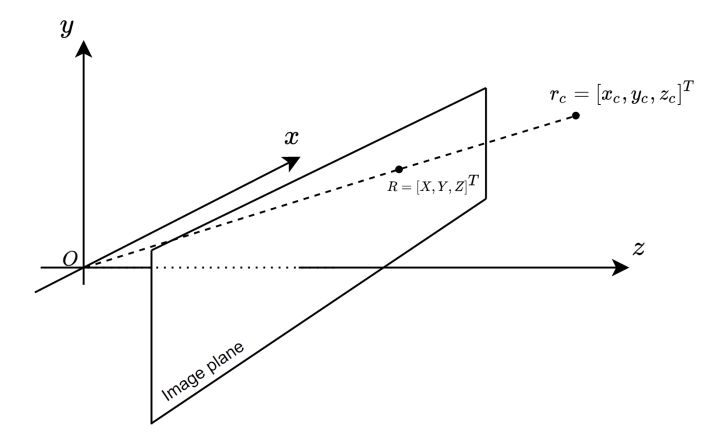
\includegraphics[width=.8\textwidth]{camera_model.jpg} 
%     \caption{相机模型} 
%     \label{相机模型} 
% \end{figure} 
\par

% \section{射频切换设计}[Content specification]
% 尽管射频与运动预测好像没有直接关系,但是射频切换确实依赖于运动预测的。
% 在RoboMaster赛场上,如何把握发弹时机是非常关键的一环。
% 对于敌方车辆在静止状态和匀速运动状态时切换到高射频模式集火攻击非常关键,
% 然而这种情况在一些场景下转瞬即时,
% 如果依赖于操作手手动切换射频往往容易错过时机,因此,选择通过视觉算法作出是否切换长高射频模式。\par

% 对于预测击打,即当敌方车辆处于非陀螺状态时,我们通过判断此时预测器预测质量的好坏来判断是否切换射频。
% 具体来说,射频默认在低射频模式,在当前图像结算出目标的世界坐标后,然后计算子弹飞行时间,
% 根据子弹飞行时间到退到历史预测器,根据历史预测器的状态对当前帧进行预测,并将预测点反投影到图像上,
% 如果反投影点在识别的装甲板矩形框之内,则认为此时预测器质量高,可以切换成高射频模式,
% 电控那边再通过判断此时云台的控制精度是否达到视觉要求的控制精度,满足条件后即可开火。
% 为了防止一些数据跳动,爆发发弹动作进入和退出都需要状态值累积到一定程度,因此设计滞回比较器,使得进入爆发发弹更加容易,退出爆发发弹更加困难。

% 然而,上述使用历史预测器来衡量当前预测器的好坏使得判断产生滞后。
% 即:子弹虚拟飞行时间太长,导致系统滞后明显。
% 那如果我选择使用临近的预测器呢?由于两个预测器相隔时间太近,导致子弹虚拟飞行时间太短,
% 即使预测器的速度信息不准确,但是由于乘以一个时间小量导致总体预测位置偏出不大,即重投影点不具有太高的可信度。
% 因此应该选择一个阈值,比如0.5s。如果通过当前目标计算的子弹飞行时间高于阈值,
% 则选择0.5s之前时刻的历史预测器计算重投影点,低于该阈值则依然采用子弹飞行时间倒推的历史预测器。




\section{运动预测效果分析}[Content specification]

至此,卡尔曼滤波器中所有输入均已确定。在实际测试过程中认知到影响运动预测效果的几个方面:
\begin{enumerate}[itemsep=2pt,topsep=0pt,parsep=0pt]
    \item 识别效果,主要包括正确识别的帧率、灯条角点回归的准确性。
    \item 运动模型建立的准确性。例如:如果物体是加速运动,那么按照匀速运动模型对物体建模就会有偏差。
    \item 噪声设置的准确性。这个影响非常的关键。卡尔曼滤波器的观测噪声和过程噪声都是需要我们手动设置的,然而这些参数是很难通过测量得到的,
    只能够采用手动调参的方式解决。观测噪声相对于测量噪声过大,会导致系统更加依赖预测值,系统跟随性能好,但是面对噪声大的数据容易不稳定,产生震荡;
    观测噪声相对于测量噪声过小,会导致系统更加依赖观测值,系统产生滞后。我得到的调参经验是,先去找一个极小值和极大值,
    然后设置参数为他们的中间值看表现效果,如表现效果更接近极小值,则更新极小值为中间值,反之则更新极大值为中间值。
    \item 目标距离。使用历史信息拟合的速度$v_x$来对未来做预测,但是前提是速度是不变的,
    否则无法利用过去的速度预测未来的位置,在预测时间$t$内,物体的运动速度是可变的,
    积分得到的位移变化量就不是$v_x*t$。然而考虑到物体惯性属性,
    在短时间内速度不会产生较大的突变,实际的位移量与计算的位移量相差不大,那还是可以击中物体的(可以理解为线性近似的误差越小)。
    \item 子弹速度。与目标距离的影响原因一致。子弹速度越大,飞行时间越短,线性近似的误差越小,命中率越高,反之命中率越低。

\end{enumerate}

\section{本章小结}[Content specification]

通过分析相机的观测模型在惯性系下建立物体的匀速运动模型,
将运动模型嵌入到卡尔曼滤波器中,且同时达到平滑数据的效果, 如图\ref{滤波}所示,蓝色为原始数据,红色为滤波之后的数据。

\begin{figure}[H]
    \centering
    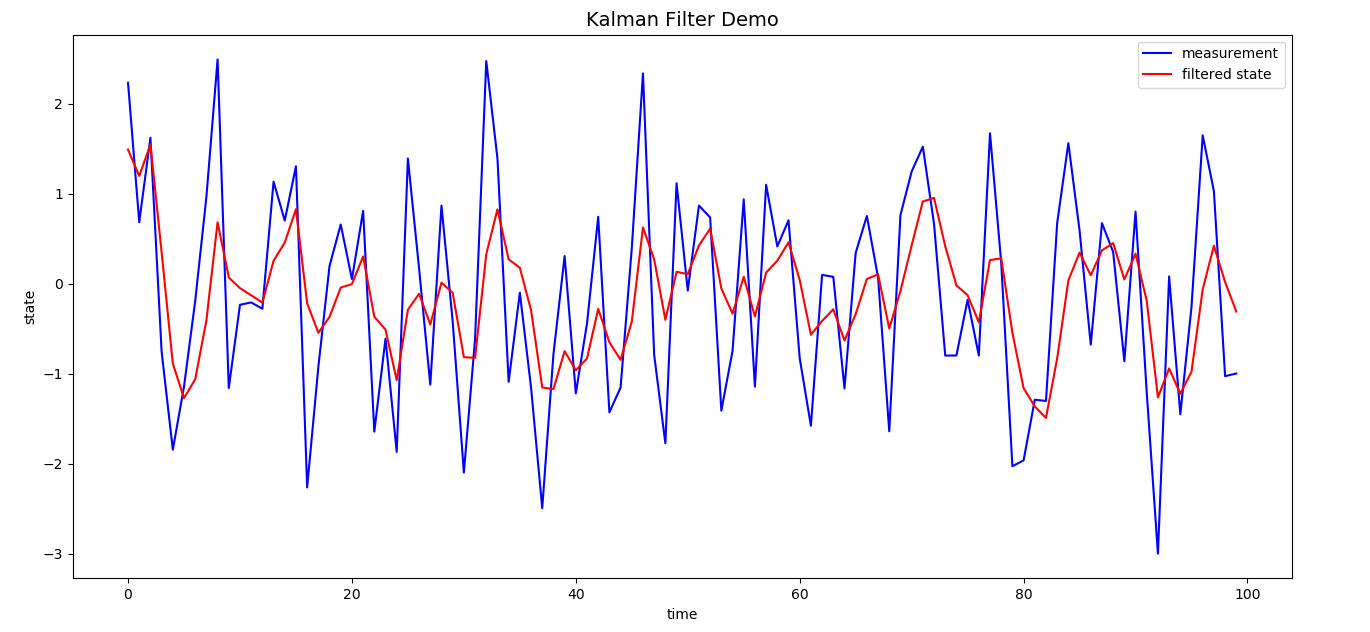
\includegraphics[width=\textwidth]{kalman_example.png} 
    \caption{卡尔曼滤波器滤波效果}
    \label{滤波} 
\end{figure}    

预测效果如下图\ref{预测效果}所示,其中红色点为预测点,白色圆圈为历史预测器对当前位置的预测,
可以看出,在物体从右向左匀速移动时,预测器效果很好,白色圆圈始终位于装甲板上,而在左侧换向时,由于非线性,
白色圆圈偏离装甲板区域,换向完成后,白色圆圈又逐渐回到装甲板上。
\begin{figure}[H]
    \centering
    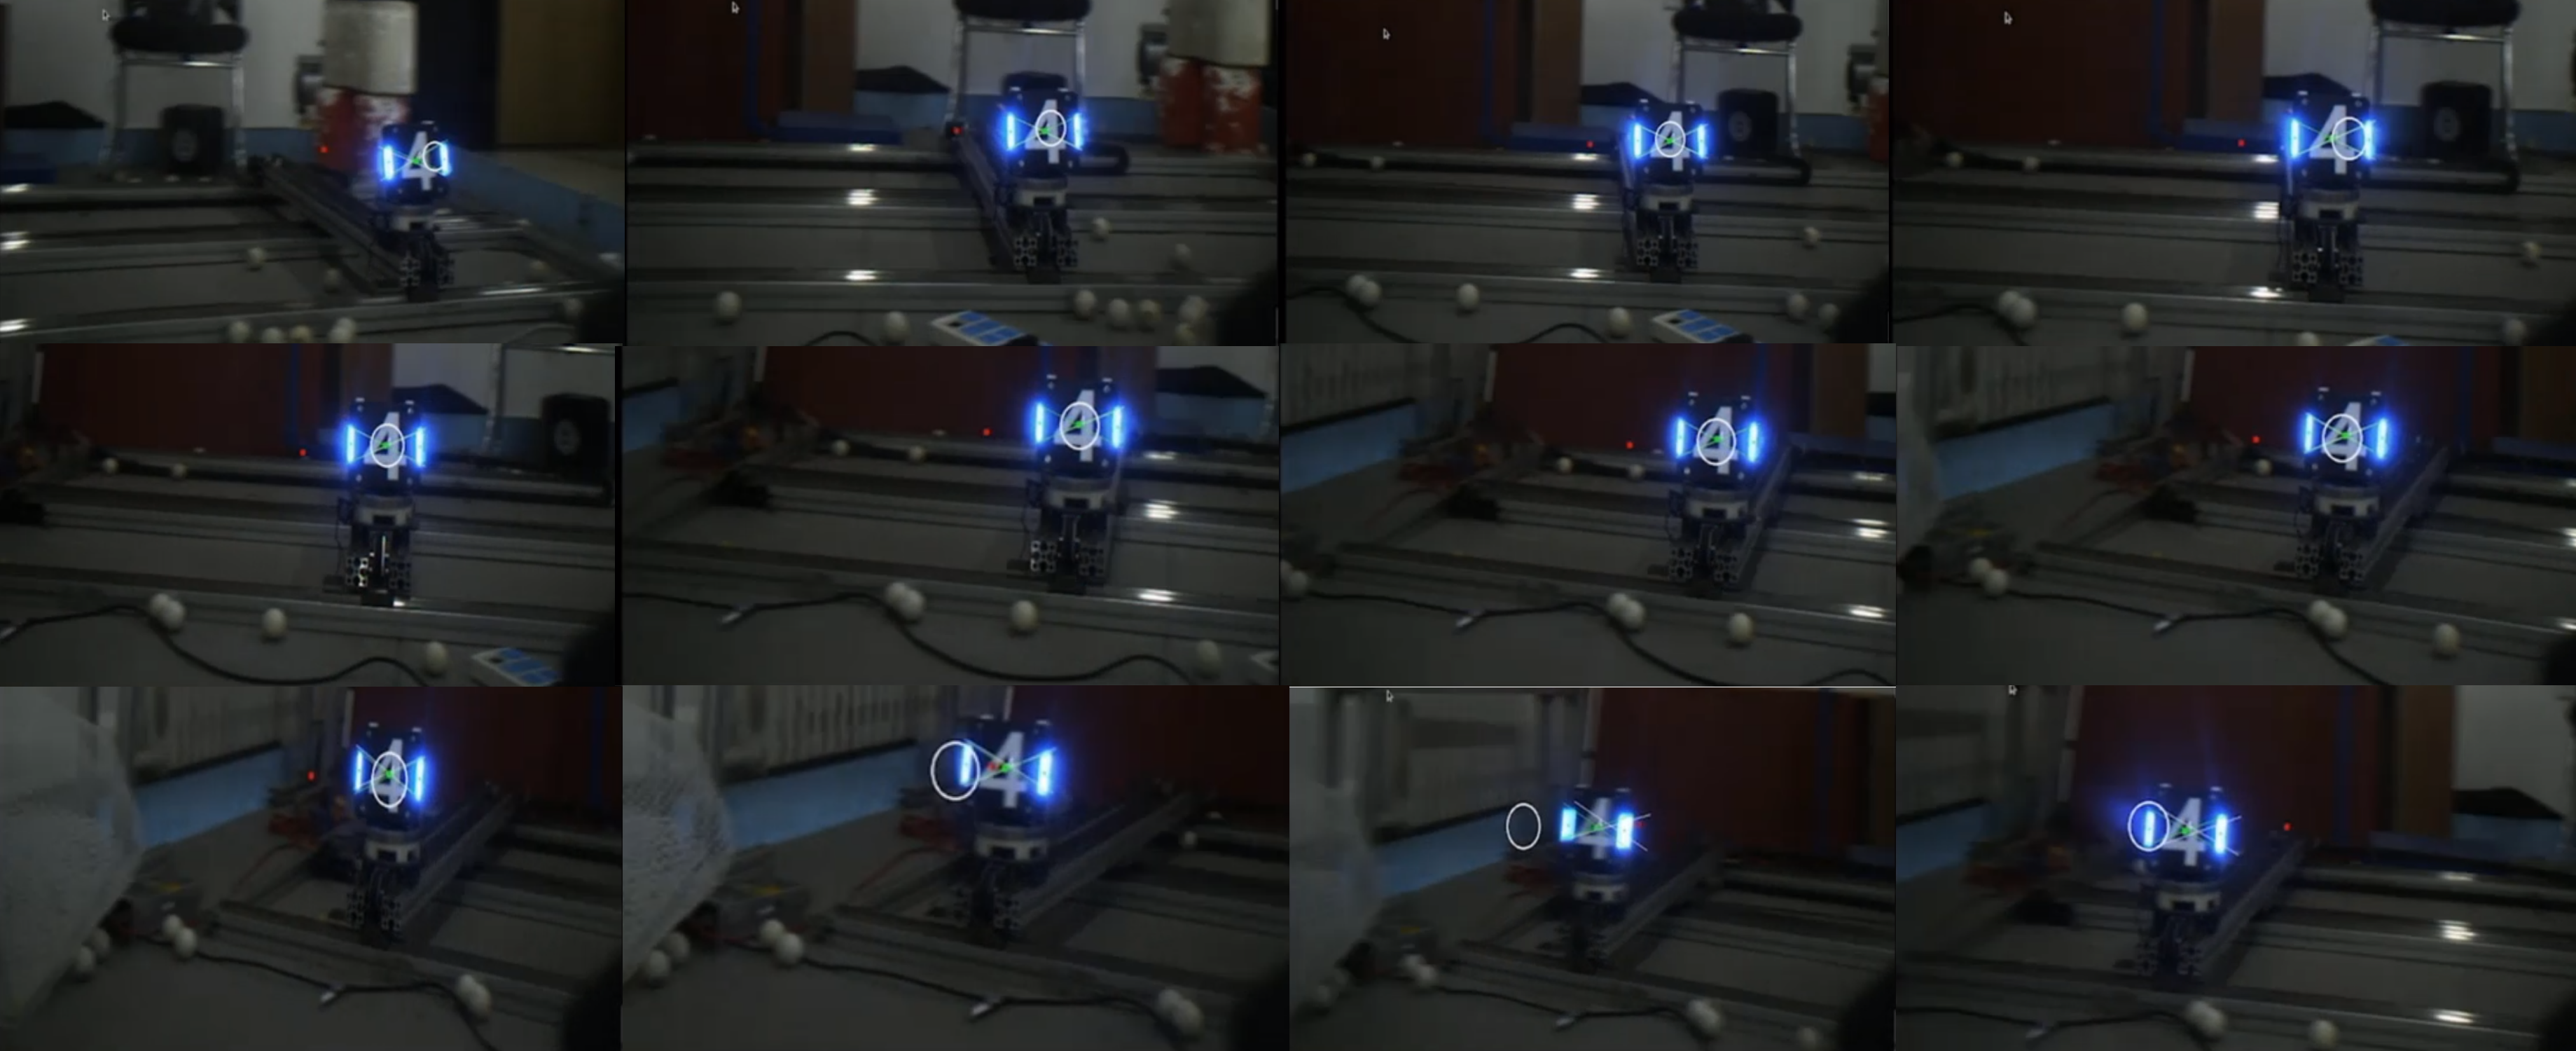
\includegraphics[width=\textwidth]{predict_demo.png} 
    \caption{运动物体预测效果}
    \label{预测效果} 
\end{figure}    